\chapter{\attekintes}

\section{Funkcionális áttekintés}

Munkám célja hogy mutasson egy olyan megközelítést, amelynek segítségével lehetséges gráfmintaillesztő
rendszerek tesztelése több aspektusból. Ezt úgy viszem véghez, hogy a rendszer nyelvén generálok
mintákat/lekérdezéseket, amelyeket aztán a lekérdező motoron futtatok. A generálásnak az az előnye,
hogy sok és diverz lekérdezést lehet így elkészíteni, ezért a nagy lekérdezéshalmaz alkalmassá válik
arra hogy teljesítményben tesztelje a lekérdező rendszereket. Illetve ha egyes lekérdezéseken nem tud
futtatni a rendszer akkor kiderül az is hogy milyen funkcionalitásokat nem fed még le. Egy 
referencia implementáció segítségével azt is ellenőrizni tudjuk, hogy a megfelelő válaszokat adja-e
a rendszer, hibás-e a működése. A megközelítésemet egy Neo4J \cite{neo4j} gráf adatbázison mutatom be 
miközben a lekérdezéseket az ehhez kifejlesztet Cypher \cite{Cypher} nyelven generálom.

Az elképzelést \aref{fig:funkcionalisAttekintes} ábrán mutatom be. A \textbf{Nyelvi specifikációt} a slizaa \cite{slizaa_2018} által készített openCypher EMF \cite{EMF} metamodell felhasználásával készítettem el. Az ott található metamodellt leszűkítettem a
Cypher nyelvű \mm{SinglePartQuery} lekérdezések metamodelljére. Az \textbf{esettanulmány szignatúráját} a trainbenchmark \cite{szarnyas2018train} által használt szignatúra felhasználásával készítettem el. A \textbf{lekérdezés generátort} bővebben a következő szekcióban mutatom be. A \textbf{generált lekérdezéseket} egyaránt futtatom a tesztelés alatt álló \textbf{lekérdező rendszeren}, illetve egy másik \textbf{referencia implementáción} is. A lekérdezések eredményeinek összehasonlításával \textbf{tesztelhetővé} válik a  \textbf{lekérdező rendszer} illetve a válaszidők összehasonlításával \textbf{teljesítmény mérést} is végezhetünk.

\begin{figure}
	\centering
	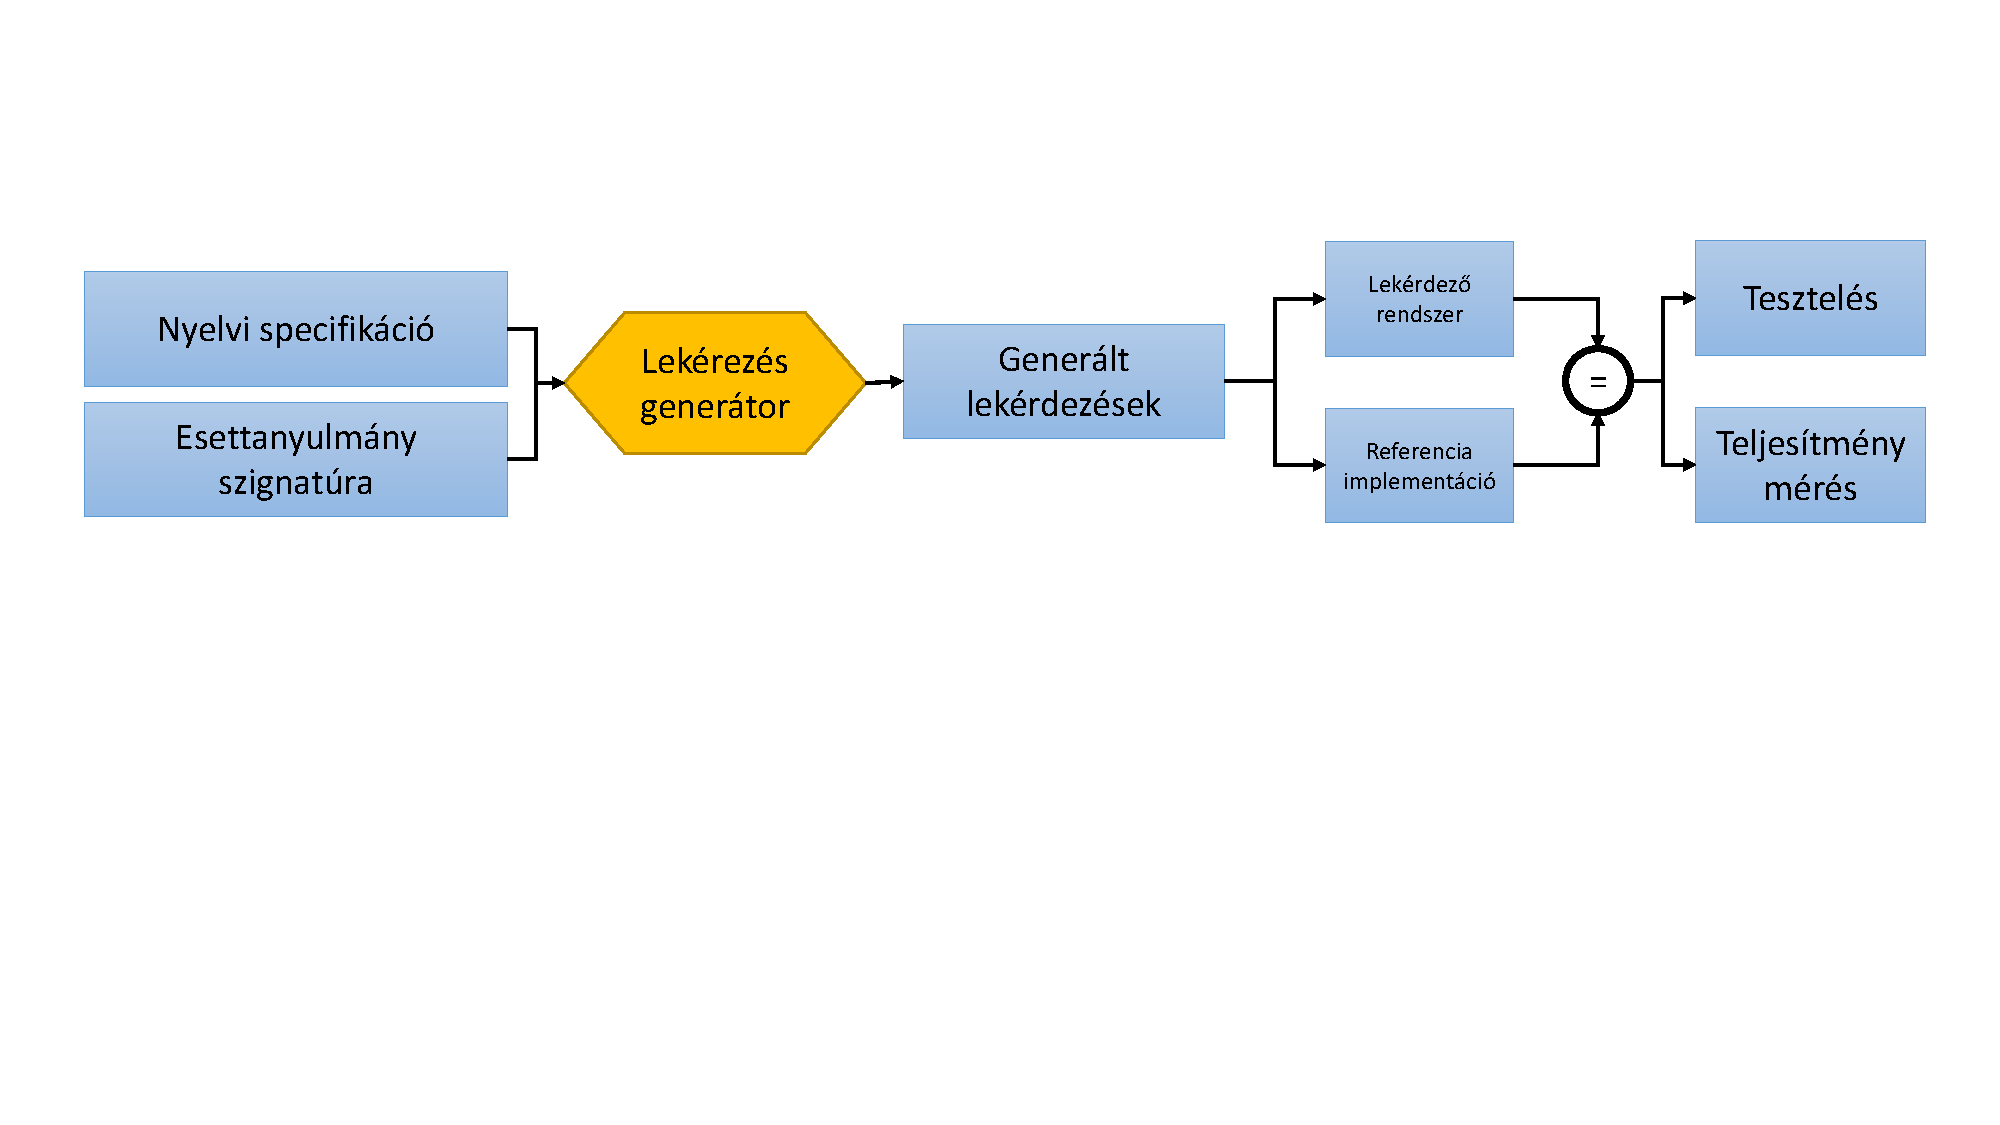
\includegraphics[width=1.0\textwidth]{figures/funkcionalisAttekintes}
	\caption{Az elképzelés funkcionális áttekintése}
	\label{fig:funkcionalisAttekintes}
\end{figure}
 
  

\section{Lekérdezés generálási folyamat felépítése}


A folyamat felépítését \aref{fig:blokkdiagramAttekintes} -es ábra segítségével ismertetem.  

\begin{figure}
	\centering
	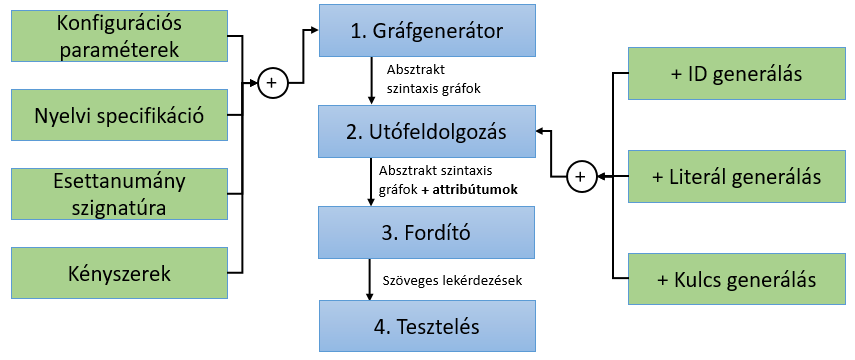
\includegraphics[width=1.0\textwidth]{figures/blokkdiagramAttekintes}
	\caption{A lekérdezés generálási folyamat áttekintése}
	\label{fig:blokkdiagramAttekintes}
\end{figure}
\begin{enumerate}
	\item \textbf{Gráfgenerátor}
	A gráf generálást a Viatra Solver keretrendszer  segítségével végzem. Ehhez sok különböző bemenetet kell megadnom. 
	\begin{enumerate}
		\item\textbf{Nyelvi specifikáció}: A Cypher nyelv specifikációját tartalmazó metamodell a nyelv egészére kiterjed. Így lekérdezéseken kívül sok egyéb műveletet is definiál, mint például létrehozás, törlés. Olyan elemeket is tartalmaz amelyek csak bonyolítják a lekérdezéseket, hogy felhasználó centrikusabban adhassák vissza a tartalmat, például a visszatérési referencia átnevezése, az adatok csökkenő sorrendbe rendezése. Ahhoz, hogy egyszerű lekérdezéseket generáljak nem szükséges ezt a hatalmas metamodellt feldolgozni, viszont egyértelműen meg kell határozni egy olyan részmodelljét, amelyből hiánytalanul előáll az egyszerű lekérdezések nyelvi specifikációja. 
		\item\textbf{Kényszerek}:Azonban vannak	olyan szabályok amelyeket a metamodell nem tud kifejezni, betartásuk nélkül viszont a generált példánygráfok nem értelmezhetőek Cypher nyelvű lekérdezésekként. Például annak meghatározása, hogy milyen változókra lehet, és milyenekre nem lehet hivatkozni a visszatérési értékben. Ezeket a szabályokat jólformáltsági kényszerekkel tartatom be. 
		\item\textbf{Konfigurációs paraméterek}: A generátor működéséhez elengedhetetlen a saját nyelvén íródott konfigurációs fájl. Itt határozható meg, hogy milyen megoldóval működjön a generálás, hogy hányat használjon az egyes elemekből a generálás során, hogy mekkora példányokat generáljon stb.  
		\item\textbf{Esettanumány szignatúra} : A generált példánygráfok változók nélkül jönnek lérte. Ahhoz, hogy egy értelmes adatbázison végezhessük el őket, fontos hogy fel legyenek fegyverezve annak az adatbázisnak a címékéivel, típusaival. Ezért hát  össze készítettem több halmaznyi szót, ami a Train benchmark által használt adatbázis címkéiből áll. 
	\end{enumerate}
	\item \textbf{Utófeldolgozás} : Az általam generált gráfokban a változóknak nem adok értéket. Megtehetném, hogy a generálás során kitöltöm őket, de csak úgy, hogy a gráfgenerátor a generált szavakat különbségekként kezelje két példánygráf között. A nagyobb diverzitás elérésének érdekében döntöttem úgy hogy üresen hagyom az értékeket.  Az utófeldolgozás során az Esettanulmány szignatúra szavaival töltöm fel az addig még csonka példánygráfokat.    
	\item \textbf{Fordító} : Az utófeldolgozás során sorosíthatóvá vált példány gráfokat a Cypher nyelv XText nyelven íródott nyelvtanának segítségével szöveges lekérdezésekké alakítom.  
\end{enumerate}



